\section{Policy Learning via Policy Iteration}
\label{appendix:policy_iteration}

We can alternatively adopt a policy iteration-based approach formulated in the following way for policy learning. The objective of training LLMs via RL can be written as a KL-constrained policy optimization problem:
\[
J(\pi)=\mathbb{E}_{\pi}\left[\sum_{h=1}^{H}\left(r(s_h,a_h)-\beta\log\frac{\pi(a_h|s_h)}{\pi_{\text{ref}}(a_h|s_h)}\right)\right].
\]
By defining the modified reward
$
\bar{r}(s,a)=r(s,a)+\beta\log\pi_{\text{ref}}(a|s),
$
we arrive at an equivalent maximum-entropy RL formulation:
\[
J(\pi)=\mathbb{E}_{\pi,s_0\sim d_0}\left[\sum_{h=1}^{H}\left(\bar{r}(s_h,a_h)+\beta\mathcal{H}(\pi(\cdot|s_h))\right)\right].
\]
Under this formulation, the Q-function and value function satisfy the soft Bellman equation:
\[
Q(s_h,a_h)=\bar{r}(s_h,a_h)+V(s_{h+1}).
\]
Given the above relationships, we can optimize the Q-function via the loss:
\[
L_Q(\theta)=\mathbb{E}_{(s_h,a_h, s_{h+1})\sim \mathcal D}\left[\left(Q_{\theta}(s_h,a_h)-\bar{r}(s_h,a_h)-V_\phi(s_{h+1})\right)^2\right].
\]
Given the estimates of Q-function and value function, the optimal policy satisfies:
\[
Q_\theta(s_h,a_h)=V_\phi(s_h)+\beta\log\pi_\theta(a_h|s_h).
\]
Substituting this optimal policy relationship back into the Bellman equation results in the following policy optimization objective:
\[
L_{\pi}(\theta)=\mathbb{E}_{(s_h,a_h,s_{h+1})\sim \mathcal D}\left[\left(V_{\phi}(s_h)+\beta\log\pi_{\theta}(a_h|s_h)-\bar{r}(s_h,a_h)-V_{\phi}(s_{h+1})\right)^2\right].
\]
Since we have estimated the advantages \(A(s_h,a_h)=V(s_{h+1})-V(s_h)\), explicit estimation of value function \(V\) is not necessary. Thus, the policy optimization objective further simplifies to:
\[
L_\pi(\theta)=\mathbb{E}_{(s_h,a_h)\sim \mathcal D}\left[\left(\beta\log\frac{\pi_\theta(a_h|s_h)}{\pi_{\text{ref}}(a_h|s_h)}-A(s_h,a_h)\right)^2\right].
\]
Each iteration of this procedure corresponds to a policy improvement step, and after updating the policy, newly sampled trajectories can be employed to update the Q-function estimation. 
% Since we explicitly reparameterize the Q-function using the policy \(\pi_\theta\), updates to the Q-function also result in an update to the policy itself. Repeating this iterative process progressively improves the policy.

We conduct preliminary experiments using this objective function, where we adopt our SPO-tree (6-6-6) method and introduce an importance weight $ \frac{\pi_\theta}{\pi_{old}} $
 to alleviate the off-policy influence. The results, shown in Figure \ref{fig:policy_iteration}, demonstrate that our approach enables steady policy improvement. 
 However, it does not reach the performance achieved by policy gradient with probability masks described in Section \ref{subsec:policy-optimization-using-edges-with-non-zero-advantage}), which achieves a validation accuracy slightly above 0.7.
 
\begin{figure}[!h]
\centering
  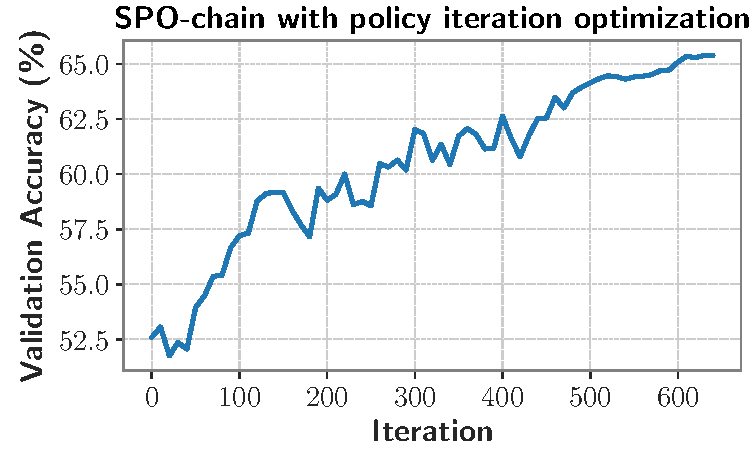
\includegraphics[width=0.55\textwidth]{eval-figures/Appendix-policy-iter.pdf}
  \caption{Validation accuracy on GSM8K using policy iteration optimizing method.}
  \label{fig:policy_iteration}
\end{figure}